\section{Auswertung}
\label{sec:Auswertung}
\subsection{Berechnung der Brechungsindices $n_i$}
\subsubsection{Berechnung des \texorpdfstring{$\upvarphi$}{phi}-Winkels des verwendeten Prismas}

Für die Berechnung der Brechungsindices ist es notwendig zunächst den Winkel $\upvarphi$ zu bestimmen.
Seine Lage kann der Abbildung \ref{fig:Phi} entnommen werden.
Die Messwerte sind in Tabelle \ref{tab:Phi} zu finden.

\begin{table}
  \centering
  \caption{Gemessene Werte für $\upvarphi_{\text{r}}$ und $\upvarphi_{\text{l}}$, sowie die berechneten $\upvarphi$-Werte}
  \label{tab:Phi}
  \sisetup{table-format=3.1}
  \begin{tabular}{S S [table-format=3.1] S [table-format=3.2]}
    \toprule
    {$\upvarphi_{\text{r}} \:/\: \si{\degree}$} & {$\upvarphi_{\text{l}} \:/\: \si{\degree}$} & {$\upvarphi \:/\: \si{\degree}$} \\
    \midrule
    79.0  & 199.0 & 60.0  \\
    209.3 & 329.5 & 60.1  \\
    198.4 & 318.5 & 60.05 \\
    201.4 & 321.4 & 60.0  \\
    180.1 & 300.2 & 60.05 \\
    223.2 & 343.3 & 60.05 \\
    216.3 & 336.3 & 60.0  \\
    \bottomrule
  \end{tabular}
\end{table}

Um nun den eigentlichen Winkel $\upvarphi$ aus $\upvarphi_{\text{r}}$ und $\upvarphi_{\text{l}}$ der Tabelle \ref{tab:Phi} zu berechnen wird die Gleichung !!!! verwendet.
Der Mittelwert der errechneten $\upvarphi$ wird mit folgender Formel berechnet:

\begin{equation}
  \label{eqn:mittelwert}
  \overline{x} = \frac{1}{N} \sum_{i=1}^N x_i
\end{equation}

Der entsprechende Fehler mittels dieser:

\begin{equation}
  \label{eqn:mittelwertfehler}
  \Delta \overline{x} = \frac{1}{\sqrt{N}} \sqrt{\frac{1}{N-1} \sum_{i=1}^N (x_i - \overline{x})^2}
\end{equation}

Die Berechnungen erfolgen mit numpy und uncertainties.
Für $\upvarphi$ ergibt sich dann folgender Wert:

\begin{align*}
  \upvarphi &= \SI{60.04 \pm 0.01}{\degree}
\end{align*}

\subsubsection{Berechnung des \texorpdfstring{$\eta$}{phi}-Winkels des parallelen Strahlenganges}

\begin{figure}
  \centering
  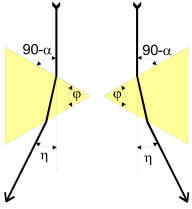
\includegraphics[scale=0.6]{images/Eta2.png}
  \caption{Der Brechungswinkel $\eta$: Aus der Anleitung des Versuches \cite[25]{1}}
  \label{fig:Eta2}
\end{figure}

\begin{table}
  \centering
  \caption{Gemessene Werte für $\Omega_{\text{r}}$ und $\Omega_{\text{l}}$}
  \label{tab:Eta}
  \sisetup{table-format=3.1}
  \begin{tabular}{S S S [table-format=3.1]}
    \toprule
    {$\text{Farbe}$} & {$\Omega_{\text{r}} \:/\: \si{\degree}$} & {$\Omega_{\text{l}} \:/\: \si{\degree}$}\\
    \midrule
    \text{rot}         & 237.1 & 119.8 \\
    \text{gelb}        & 236.7 & 120.2 \\
    \text{hellgrün}    & 236.4 & 120.6 \\
    \text{grün}        & 235.8 & 121.1 \\
    \text{hellblau}    & 235.3 & 121.6 \\
    \text{blau}        & 235.1 & 121.9 \\
    \text{hellviolett} & 234.3 & 122.7 \\
    \text{violett}     & 233.3 & 123.7 \\
    \bottomrule
  \end{tabular}
\end{table}
